% TODO: could use some high level diagram of the method at the start of the
% section (acting as a bit of a map)?
% TODO: in general, more assertive language would be good. 

% TODO: kinda want to improve the sampling figure

Our proposed method aims to push the efficiency of generative models to the
limit via a combination of current techniques. To do so, we first use pretrained
\glspl{vqgan} models from~\cite{esser2021taming} to generate a dataset of
discrete latent representations, described in \S\ref{subsec:datasetGen}. By
operating at a latent level, we reduce the spatial resolution for our second
stage generator. We implement our generator as a modified hourglass transformer,
described in \S\ref{subsec:improvedHourglass} and trained using a \gls{nar}
method described in \S\ref{subsec:sundaeTraining}. This permits extremely fast
sampling described in \S\ref{subsec:sundaeSampling}. To thoroughly test the
efficiency and scalability of our approach, we train a megapixel \gls{vqgan}
(described in \S\ref{subsec:megagan}) and repeat \gls{sundae} training and
sampling on the resulting discrete latent representations. In
\S\ref{subsec:inpainting}, we explore flexible inpainting using our framework.

Each component represents the pinnacle of performance in their respective areas:
compression ratio in \gls{vq} image models with \gls{vqgan}, fast \acrlong{nar}
sampling of discrete data with \gls{sundae}, and transformer scalability with
our modified hourglass transformer. Together, we obtain an extremely efficient
generative model that permits sampling at $1024 \times 1024$ resolution in mere
seconds.

\subsection{Latent Dataset Generation}
\label{subsec:datasetGen}

We use the standard two-stage scheme for vector-quantized image
modelling~\cite{oord2018neural,razavi2019generating,esser2021taming,bondtaylor2021unleashing}
using \gls{vqgan}~\cite{esser2021taming} as our feature extractor. Where such
models are available, we use pretrained \glspl{vqgan} for our experiments. For
higher resolution experiments (for example,
FFHQ1024~\cite{karras2019stylebased}), pretrained models are not available and
so the training our own VQ-GAN was necessary (see \S\ref{subsec:megagan}). 

The second stage is to train a discrete prior model over the extracted latent variables.
To enable this, we first built a latent dataset using our trained \gls{vqgan}.
This allows for faster training of our second-stage model as the discrete latent
representations have been precomputed. A downside of this approach is that it
limits the amount of data augmentation that can be applied to the dataset. We
apply a simple horizontal flip to all images, effectively doubling the dataset
size, with no other augmentation. Formally, given a dataset of images
$\imageDataset$, a \gls{vqgan} encoder $\vqganEncoder$ with downsample factor
$\vqganDownsample$, and \gls{vq} codebook $\vqganCodebook$ with
number of codewords $\vqganNbLatents$, trained on $\imageDataset$, we define our
latent dataset $\latentDataset$ as:
\begin{equation}
    \latentDataset = \{\vqganCodebook(\vqganEncoder(\image)) \mid \image \in \imageDataset \}
\end{equation}
where $\image \in \real{3 \times H \times W}$ is a single element of the
augmented image
dataset and $\latent = \vqganCodebook(\vqganEncoder(\image)) \in \{1, \dots,
\vqganNbLatents\}^{h \times w}$ is the corresponding discrete latent
representation. In other words, each $\vqganDownsample \times \vqganDownsample$
pixels in $\image$ is mapped to a single discrete value from $1$ to
$\vqganNbLatents$ (which in turn, corresponds to a vector $\codebookVector \in
\vqganCodebook$),
resulting in a latent representation of shape $\frac{H}{f} \times \frac{W}{f} =
h \times w$.

We then use $\latentDataset$ to train a discrete prior over the latents. Coupled
with the \gls{vqgan} decoder $\vqganDecoder$, we obtain a powerful generative
model by first sampling from a discrete uniform prior distribution, iteratively
denoising using \gls{sundae}, and then decoding the final latents using the
\gls{vqgan} decoder. The training this discrete prior model, forms the bulk of our
work in this paper.

\subsection{2D-Aware Hourglass Transformer}
\label{subsec:improvedHourglass}

Inspired by successes in hierarchical transformers for generative language
modelling~\cite{nawrot2021hierarchical}, we modify their architecture for use
with discrete latent representations of image data. We will later use this
architecture to implement a discrete prior over the \gls{vqgan} latents. 

Hourglass transformers have been shown to efficiently handle long-sequences,
outperform existing models using the same computational budget, and meet the
same performance as existing models more efficiently by using an explicit
hierarchical structure~\cite{nawrot2021hierarchical}. The same benefits should
also apply to vector-quantized image modelling. 

However, the design and parameters chosen by the original authors were tailored
for language modelling~\cite{nawrot2021hierarchical}. They also experimented
with pixel-wise image generation, though we believe that we can improve upon
their architectural choices for the task of discrete latent modelling. Some
changes may also be applicable to pixel-level generation. In this subsection,
modifications to the architecture are outlined.

\textbf{2D-Aware Downsampling} -- The original formulation of hourglass
transformers~\cite{nawrot2021hierarchical} introduced both upsampling and
downsampling layers, allowing the use of hierarchical transformers in tasks that
have output sequence lengths equal to the input sequence lengths. However,
we found certain flaws in their original formulation that hinders performance on
multi-dimensional inputs.

In their work, resampling is applied to the flattened embedding sequences,
meaning that a corresponding two-dimensional vector-quantized image is resampled
more in one axis compared to the other. In their work they did not address this,
except for experiments on ImageNet32~\cite{russakovsky2015imagenet} where they
resampled with a rate of $\hourglassRate=3$, corresponding to three colour
channels. However, if they were to resample again by nesting the hourglass
transformers, issue of one spatial dimension being
downsampled more than others would then occur.

\begin{figure}[ht!]
    \label{fig:resample}
    \centering
    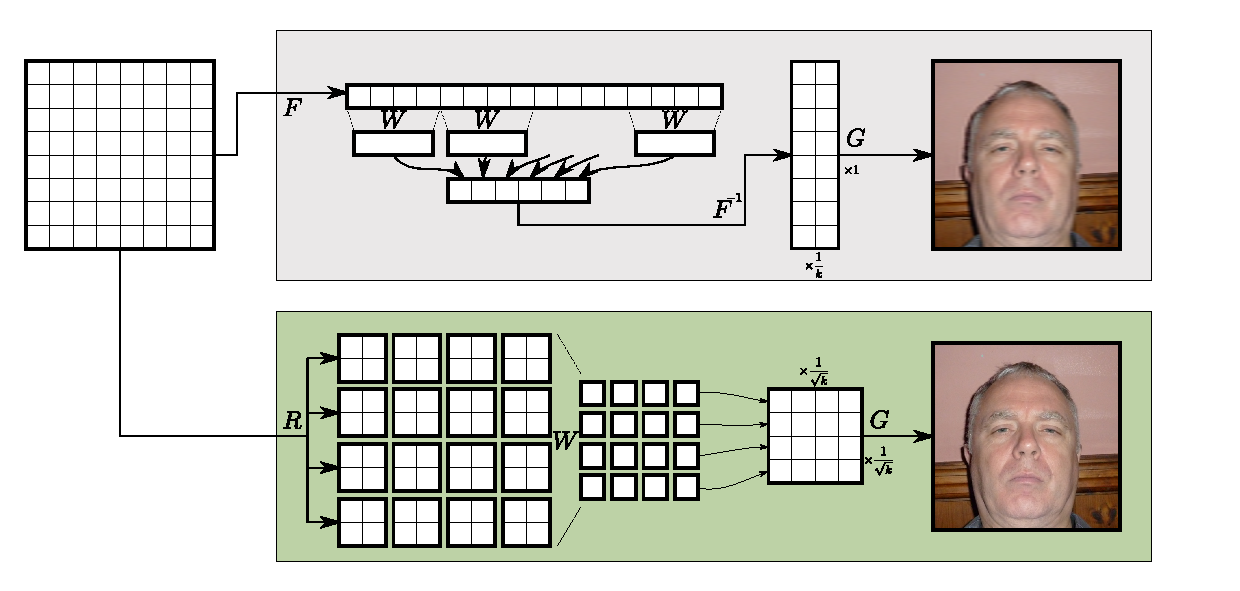
\includegraphics[width=\textwidth]{figures/resample.pdf}
    \caption{
        \textbf{Top:} Showing effect of resampling sequence embeddings using
        original formulation. Resampling rate will be applied to only one axis,
        resulting in resampling more in only one axis of the decoded image.
        \textbf{Bottom:} Our corrected method of resampling, extracting first
        two-dimensional patches of size $\sqrt{\hourglassRate}$, then applying
        resampling. The sequence is then again be flattened and passed to
        subsequent transformer layers.
    }
\end{figure}

In our formulation, we instead reshape the flattened sequence back into its a
two-dimensional formulation and then apply resampling equally in the last two axes.
With a resampling rate of $\hourglassRate$ we apply $\sqrt{\hourglassRate}$ in
each axis -- evenly distributing the resampling among the axes. In our
preliminary experiments, we found this to significantly improve the performance
of the discrete prior model, and suspect a similar approach could improve
performance if applied to pixels directly, which we leave for future work to
confirm.

For all experiments, we use the linear resampling method proposed
in~\cite{nawrot2021hierarchical} as this was the recommended option for image
data. In addition, attention layers are applied directly after resampling as
this led to best results on both image and text datasets in the original
work~\cite{nawrot2021hierarchical}. This means our adjusted resampling method is
as follows:
\begin{equation}
    h' = A(\hourglassResample^{(\intercal)} \cdot R(\vh) + \vr), \;\; \hourglassResample \in
    \mathbb{R}^{\frac{(d \cdot h \cdot w)}{\hourglassRate} \times (d \cdot h \cdot w)}
\end{equation}
where $A$ is the post-resampling attention layer, $\vh$ is the current hidden
state, $\vr$ is the residual (with $\vr = \bm{0}$ when downsampling), $R$ is the
modified reshape operation, $d$ is the hidden layer dimension, and $W$ is a
learned projection matrix. The reshape operation $R$ was implemented as a
space-to-depth operation followed by combining the feature and depth dimensions.

\textbf{Rotary Positional Embeddings}~\cite{su2021roformer} are a good default
choice for injecting positional information into transformer models, requiring
no additional parameters. Additionally, they can be easily extended to the
multi-dimensional case~\cite{rope-eleutherai} which we exploit here. Though
transformers are clearly capable of learning that elements far apart in a
flattened sequence may be close in a multi-dimensional final output, we found
that explicitly extending positional embeddings to the multi-dimensional case to
provide a modest boost in performance and improve the rate of training
convergence. The original hourglass transformer on pixel-wise generation also
opted to use rotary embeddings~\cite{nawrot2021hierarchical}. They note also
that rotary embeddings have the advantage of being compatible with any
self-attention mechanism.

\textbf{Removal of Causal Constraints} -- In the original autoregressive
formulation of hourglass transformers, great care was taken to avoid information
leaking during resampling, and hence making the model
non-causal~\cite{nawrot2021hierarchical}. We use a non-autoregressive method
which is therefore not causal. Hence, in our approach we do not make any special
considerations to avoid information leaking into the future. This simplifies the
model by avoiding ``shifting'' and causal masking operations required in the original work.

\subsection{Training a megapixel VQ-GAN}
\label{subsec:megagan}

\begin{figure}[ht]
    \label{fig:recon}
    \centering
    \includegraphics[width=\textwidth]{figures/recon.pdf}
    \caption{
        \gls{vqgan} does not produce entirely faithful reconstructions due to
        being optimised for perceptual quality rather than a direct error between
        the reconstructions and inputs. The top row shows example inputs, middle row
        shows resulting reconstructions, and the final row shows points of interest that
        have been modified -- some perceptually valid and others clear
        artifacts. 
        \textbf{Left}: The eye colour has been brightened, and hair
        shifted to conceal a piercing, rather than reconstruct it.
        \textbf{Middle}: The most common reconstruction artifact occurs with
        certain types of hair, where a repeating and unrealistic pattern occurs. The
        pose of the lip is also altered. 
        \textbf{Right}: Another common artifact where text in images is
        corrupted. This is common across many generative models. Additionally,
        the model removes nose and lip piercings, in addition to altering eye
        makeup. This is again a valid image, but does not faithfully reconstruct
        the input.}
\end{figure}

Training at higher resolutions means greater computational requirements and
sampling speeds. With an autoregressive model, the sampling speed can be
especially immense as it scales linearly with data dimensionality, even with an
auxiliary vector-quantized image model~\cite{esser2021taming}. With a
non-autoregressive model however, the sampling speed is explicitly controlled
and does not directly grow as a function of input size -- excluding the
increase in time for one network pass from using a larger model on a larger input.

We trained a larger variant of \gls{vqgan} with $\vqganNbLatents = 8192$ operating on
$1024 \times 1024$ RGB images. To our knowledge, this is the highest resolution
dataset \gls{vqgan} has been applied to~\cite{esser2021taming}. Once trained,
we generate a latent datasets as before, the only difference being an increased
sequence length -- greater than was ever tested in the original
work~\cite{savinov2022stepunrolled}. Specifically, we obtain a downsampling rate
of $\vqganDownsample=32$, resulting in discrete latent size of $32 \times 32 =
1024$.

The resulting reconstructions are overall of good quality given the relatively
extreme compression ratio we are using. However, certain artifacts in the
reconstructions still remain. Figure \ref{fig:recon} shows examples of
particularly prevalent artifacts including occasional unrealistic textures in
hair (middle reconstruction) and corruption of text (right reconstruction). The
corruption of text is a common issue in \gls{vq} image
models~\cite{ramesh2021dalle}, and the unrealistic textures are a result of the
extreme compression rate or a simple lack of model capacity.

\Gls{vqgan} is trained to minimise the true error, perceptual loss, and an
adversarial loss~\cite{esser2021taming} in addition to a $k$-means \gls{vq}
loss. In our implementation, \gls{vqgan} is trained to minimise the following
loss:
\begin{align}
\begin{split}
    L_\text{PIX} &= \alpha_\text{PIX} \cdot |\image - \hat{\image}| \cdot \\
    L_\text{VQ} &= \alpha_\text{VQ} \cdot \left(||\hat{\latent} -
    \latent||^2 + ||sg[\vqganEncoder(x)] - \latent||^2_2 + ||\vqganEncoder(x) -
    sg[\latent]||^2_2\right)\\
    L_\text{GAN} &= \alpha_\text{GAN} \cdot \left(\log D(x) + \log
    (1-D(\hat{x}))\right) \\
    \lambda &= \frac{\nabla_{G_{-1}}[L_\text{PIX} +
    L_\text{PER}]}{\nabla_{G_{-1}}[L_\text{GAN}] + \epsilon}\\
    L &= L_\text{VQ} + \lambda \cdot L_\text{GAN}\\
    \alpha_\text{PIX} &= 1.0,\; \alpha_\text{VQ} = 1.0,\; \alpha_\text{GAN} = 0.5,\; \alpha_\text{PER} = 1.0
\end{split}
\end{align}
\cite{esser2021taming} where our discriminator is implemented using three
layers, perceptual loss $L_\text{PER}$ implemented using a pretrained VGG16
model~\cite{karen2014vg18}, $\nabla_{G_{-1}}[\cdot]$ is the gradient with
respect to the last layer of the \gls{vqgan} decoder $\vqganDecoder$, and
$sg[.]$ is the stop-gradient operator. The
generator and discriminator model parameters are updated separately, as is
standard procedure in \gls{gan}-based literature~\cite{esser2021taming}.

This means there is less of a weight on directly minimising the pixel-wise error
between the input and reconstruction. This gives rise to an interesting property
of \gls{vqgan} where the reconstructions may be perceptually valid but clearly
distinct from the input. The left reconstruction in Figure \ref{fig:recon}
demonstrates this with a change in eye colour and a shift in hair position --
concealing an ear piercing. This even more apparent in the right reconstruction
where all piercings are flawlessly removed -- along with adjustments to eye
makeup.

Using \gls{vq} image models to compress images further whilst retaining high
quality and faithful reconstructions remains an open and challenging area of
research. In our case at very high resolutions, this is especially true. In our
preliminary experiments, we found a higher $\vqganDownsample$ led to the vast
majority of reconstructions being of an untenable quality. Conversely, decreasing
$\vqganDownsample$ led to latent representations of sizes that led to large
memory requirements in the downstream \gls{sundae} prior, making inference on
consumer-grade GPUs impractical.

Training \gls{vqgan} at this resolution and our chosen downsampling rate is
extremely computationally expensive -- in our configuration we were limited to a
global batch size of 4 across four, 32GiB Tesla V100 GPUs. This made a full
hyperparameter sweep of the other parameters of the model not possible.
Therefore, we accepted good reconstructions on average with occasional
artifacts that could potentially manifest in the final samples. Improving the
effectiveness \gls{vq} image model itself is not the focus of this research
project. Ultimately, we found these artifacts to only appear rarely in the final
samples, shown in \S\ref{subsec:evaluationUnconditional}.

\subsection{Non-Autoregressive Generator Training}
\label{subsec:sundaeTraining}

We train a \gls{sundae} model on the flattened (in a raster-scan format)
extracted \gls{vq} latents $\latent = \{\latent^{(0)}, \dots, \latent^{(N)}\}$
where $N = \latentHeight \cdot \latentWidth$. The function $\sundae(\cdot)$ is
implemented using our proposed 2D-aware hourglass transformer. 

Given a latent $\latent$, we first apply our corruption distribution. This is
done by first sampling a corruption threshold vector $\corruptionThreshold$ with
$\corruptionThreshold_i \sim U[0, 1]$ and a random matrix $\mathbf{R}$ of the
same shape as $\latent$ where $R_{i,j} \sim U[0,1]$. Using this, we construct a
mask matrix $\mathbf{M}$ with $M_{i,j} = 1$ when $R_{i,j} < t_i$ and $0$
otherwise. This results in $\mathbf{M}_i$ having approximately
$\corruptionThreshold_i$ of its entries be $1$.

Then, given $\latent_0 \sim p_0$, we compute a new $\latent_0$ to start unrolled
denoising from:
\begin{equation}
    \latent_0 \leftarrow \mathbf{M} \cdot \latent_0 + (\mathbf{1} - \mathbf{M})
    \cdot \latent \text{.}
\end{equation}
where $\latent$ is sampled from our latent dataset $\latentDataset$.

We then iteratively unroll the current sample $\latent_{t-1}$ to obtain
$\latent_t$ for steps $t\in \{1, \dots, \markovSteps\}$. To perform one unroll
step, simply compute logits $\sundae(\latent_t \vert \latent_{t-1})$ and then
sample from the resulting distribution to obtain $\latent_t$, storing the logits
at each step. Then, compute the cross entropy loss between all logits at each
$t$ and the target $\latent$. This differs from some other \gls{nar} solutions
which predict the corruption noise $\epsilon$~\cite{ho2020ddpm} rather than the
target itself. The mean of the cross entropy losses is then computed to produce
the final loss: 
\begin{equation} 
    \lossFunction{1:T} = \frac{1}{T} \left(\lossFunction{1} +
    \dots + \lossFunction{T} \right) 
\end{equation} 
as in \S\ref{subsec:sundae}, which then allows for backpropagation of gradients
and consequently the updating of parameters $\sundaeParameters$. Though the
default $\markovSteps = 2$ performed well, we found $\markovSteps = 3$ to result
in more diverse samples.

All models are trained using the Adam optimizer~\cite{kingma2014adam} as
realised in its AdamW implementation in PyTorch~\cite{paszke2019pytorch}.
Similarly, all models and training scripts are implemented in PyTorch. For
unconditional generation on $256 \times 256$ images, training was done on a
single 24GiB Nvidia RTX TITAN GPU. For unconditional generation on $1024 \times
1024$ images, training was done on a single 32GiB V100 GPU. Finally, for
conditional generation on ImageNet, training was done on a single 80GiB A100
GPU.

\begin{table}
    \centering
    \begin{tabular}{|c||c c||c||c c||c||}
    \hline
    \textbf{Dataset} & \textbf{FFHQ-256} & \textbf{FFHQ-1024} & \textbf{CelebA}
                     & \textbf{MNIST} & \textbf{FashionMNIST} &
                     \textbf{ImageNet} \\
    \hline
    Dataset Size & $60,000$ & $60,000$ & $190,000$ & $60,000$ & $60,000$ & $1.28$M \\
    Codebook Size & $1024$ & $8192$ & $1024$ & $256$ & $256$ & $1024$ \\
    Latent Shape & $16 \times 16$ & $32 \times 32$ & $16 \times 16$ & $28 \times
                 28$ & $28 \times 28$ & $16 \times 16$ \\
    Unroll Steps & 3 & 3 & 3 & 2 & 2 & 3 \\
    \hline
    Depth & $3-10-3$ & $2-12-2$ & $2-12-2$ & $2-8-2$ & $2-8-2$ & $3-14-3$\\
    Dimension & 1024 & 1024 & 1024 & 1024 & 1024 & 1024 \\
    Shorten Factor & 4 & 4 & 4 & 4 & 4 & 4 \\
    Attention Heads & 8 & 8 & 8 & 8 & 8 & 12 \\
    Resample Type & Linear & Linear & Linear & Linear & Linear & Linear \\
    \hline
    Classes & -- & -- & -- & 10 & 10 & 1000 \\
    Class Dimension & -- & -- & -- & 1024 & 1024 & 1024 \\
    \hline
    \end{tabular}
    \caption{
        Table of parameters for all training experiments. Depth is
        represented as three numbers corresponding to number of layers before
        downsampling, number of downsampled layers, and number of layers after
        upsampling. The dataset size is the size of the training split of the
        dataset. The latent shape of MNIST experiments is exactly equal to the
        shape of $\image$, as for these experiments we operate directly on a
        (discretized) pixel-level.
    }
\end{table}
An alternative corruption distribution would be to instead use a deterministic
method $\latent_0^{(i)}=\texttt{[MASK]}$, essentially replacing all tokens with
$M_{i,j} = 1$ with a special masking token. This bears some similarity to
``progressive unmasking'' of latents as shown in prior
work~\cite{bondtaylor2021unleashing,austin2021structured}. This strategy was not
considered due to the use of a masking token places an upper bound on the number of
inference time sampling steps (updating at most one token per step) as well as
not allowing for self-correction, as once a token is unmasked it is now
fixed~\cite{bondtaylor2021unleashing,austin2021structured}. 

% TODO: a figure could be really nice too.

\subsection{Generating High-Resolution Images}
\label{subsec:sundaeSampling}

\begin{figure}[ht]
    \label{fig:sampling}
    \centering
    %\includegraphics[width=0.9\linewidth]{figures/sampling/sampling.pdf}
    \begin{overpic}[percent,grid=false,tics=2,width=0.9\linewidth]{figures/sampling/sampling.pdf}
        \put(6, 3){\tiny$\latent_0 \sim U(1, v)$}
        \put(31, 3){\tiny$\latent_1$}
        \put(66, 3){\tiny$\latent_{T-1}$}
        \put(88, 3){\tiny$\latent_T$}
        \put(10, 31){$\vqganDecoder$}
        \put(31, 31){$\vqganDecoder$}
        \put(67, 31){$\vqganDecoder$}
        \put(88, 31){$\vqganDecoder$}
        \put(48, 16){$\dots$}
        \put(9, 60){\tiny$\sample_0$}
        \put(31, 60){\tiny$\sample_1$}
        \put(67, 60){\tiny$\sample_{\markovSteps - 1}$}
        \put(88, 60){\tiny$\sample_\markovSteps$}
    \end{overpic}

    \caption{The sampling process. SUNDAE gradually denoises from $\latent_0$ to
    the final sample $\latent_\markovSteps$. At each step, it is possible to
    decode with $\vqganDecoder$ to produce a final image. By doing so, it
    reveals the model gradually denoises the latent $\latent$ and is capable of
    correcting errors accumulated during sampling.}
\end{figure}

During sampling, we simply sample sequentially $\latent_t \sim \sundae(\latent_t
\vert \latent_{t-1})$ for a constant number of steps $\markovSteps$, beginning
randomly from $\latent_0$~\cite{savinov2022stepunrolled}. The original work
proposed a number of improved strategies for sampling in smaller number of
steps, including low-temperature sampling and updating a random subset of
tokens~\cite{savinov2022stepunrolled}, rather than all simultaneously.

Sampling, however, with a lower temperature reduces the diversity of the
resulting samples. To alleviate this, we instead anneal the temperature down
from a high value ($\approx 1.0$) down to a lower value towards the end of the
sampling process. We found this retained the fast sampling speed whilst also
improving diversity.

In certain latent sampling configurations, updating only a random subset of
tokens also helps improve diversity. \cite{savinov2022stepunrolled} used this
strategy when performing low-temperature sampling. However, we found that for
low-step sampling ($\markovSteps<20$) that all tokens must be able to be updated
in order to produce meaningful samples before the maximum number of steps is
reached. Hence in these cases, we do not follow this strategy and instead opt
for a high sample proportion. In scenarios where we are permitted a time-budget
allowing for a large number of sample steps, the sample proportion can be freely
reduced for an increase in sample diversity.

Additionally, if a individual sample does not change between step $t-1$ and $t$,
it is prevented from being changed further. If all samples are frozen, sampling
terminates early, provided a minimum number of steps have been completed. This
improves the sampling speed further with little cost to the final quality. This
is significant when performing large-batch sampling or when the maximum number
of steps is large.

Once sampling has terminated, the sampled latent code $\latent_T$ is given
to the \gls{vqgan} decoder $\vqganDecoder$ to produce a final sample $\sample$. In
fact, any $\latent_i$ in the Markov chain is a valid input to the \gls{vqgan}
decoder model. Decoding during this process and comparing the $\sample_i$
produced at each step reveals the model gradually denoises the latent and does
indeed self-correct errors accumulated during the sampling process.

\subsection{Arbitrary Pattern Inpainting}
\label{subsec:inpainting}

As noted in the original work~\cite{savinov2022stepunrolled} and other
non-autoregressive solutions~\cite{bondtaylor2021unleashing}, one clear
advantage of non-autoregressive models is that they are not limited to causal
inpainting. In general, they support arbitrary inpainting masks which draw upon
context from both the past and the future, enabling them to easily perform
inpainting tasks that are more complex to implement with autoregressive models.
This property also allows for higher quality and more diverse
samples~\cite{bondtaylor2021unleashing}.

The inpainting procedure, takes an image $\sample \in \real{H \times
W \times 3}$ and a pixel-level binary mask $\pixelMask \in \{0, 1\}^{H \times
W}$ as input. By taking $\vqganDownsample \times \vqganDownsample$ regions of
$\pixelMask$ and applying a logical \texttt{AND} in them, we obtain a latent
level mask $\vqMask \in \{0,1\}^{h \times w}$. We then sample as normal from the
latents, allowing the model full context, but only update regions that were
masked according to $\vqMask$. Like with sampling, we then use $\vqganDecoder$
to decode the sampled latent code, producing the output $\sample$.

Sampling at a latent-level means the model is unable to do fine-grained
inpainting at a pixel level. The definition of the \gls{vq} mask $\vqMask$ means
that some pixels outside the mask may also be altered if the pixel mask is not
perfectly aligned with the \gls{vq} mask. We found in practise this had little
effect on the perceptual quality of the outputs.
